\documentclass[UTF8,a4paper,zihao=-4]{ctexart}
\usepackage[margin=2.4cm]{geometry}
\usepackage{graphicx}
\usepackage{float}
\usepackage{booktabs}
\usepackage{array}
\usepackage{hyperref}
\usepackage{xcolor}
\usepackage{caption}
\usepackage{enumitem}
\usepackage{amsmath}
\usepackage{titlesec}
\usepackage{fancyhdr}
\usepackage{tikz}
\usetikzlibrary{arrows.meta,positioning,shapes.geometric}

\graphicspath{{./figures/}{./}}
\setlength{\parindent}{2em}
\setlength{\parskip}{0.35em}
\linespread{1.25}
\captionsetup{font=small,labelfont=bf}
\titleformat{\section}{\centering\bfseries\zihao{3}}{\thesection}{1em}{}
\titleformat{\subsection}{\bfseries\zihao{-3}}{\thesubsection}{0.8em}{}
\titleformat{\subsubsection}{\bfseries\zihao{4}}{\thesubsubsection}{0.8em}{}
\pagestyle{fancy}
\fancyhf{}
\setlength{\headheight}{14.5pt}
\fancyhead[C]{软件度量实验报告}
\fancyfoot[C]{\thepage}

\newcommand{\img}[2]{%
\begin{figure}[H]
  \centering
  \includegraphics[width=0.93\linewidth]{#1}
  \caption{#2}
\end{figure}}
\newcommand{\twobytwo}[5]{%
\begin{figure}[H]
  \centering
  \begin{minipage}{0.48\linewidth}\centering\includegraphics[width=\linewidth]{#1}\end{minipage}\hfill
  \begin{minipage}{0.48\linewidth}\centering\includegraphics[width=\linewidth]{#2}\end{minipage}

  \vspace{0.25em}
  \begin{minipage}{0.48\linewidth}\centering\includegraphics[width=\linewidth]{#3}\end{minipage}\hfill
  \begin{minipage}{0.48\linewidth}\centering\includegraphics[width=\linewidth]{#4}\end{minipage}
  \caption{#5}
\end{figure}}
\newcommand{\twopics}[3]{%
\begin{figure}[H]
  \centering
  \begin{minipage}{0.48\linewidth}\centering\includegraphics[width=\linewidth]{#1}\end{minipage}\hfill
  \begin{minipage}{0.48\linewidth}\centering\includegraphics[width=\linewidth]{#2}\end{minipage}
  \caption{#3}
\end{figure}}
\newcommand{\flowbox}{%
\begin{figure}[H]
\centering
\resizebox{0.98\linewidth}{!}{%
\begin{tikzpicture}[font=\normalsize, >=Latex, node distance=8mm and 9mm,
  box/.style={draw, rounded corners, align=center, minimum height=9mm, text width=3.0cm},
  mid/.style={draw, rounded corners, align=center, minimum height=9mm, text width=3.5cm},
  wide/.style={draw, rounded corners, align=center, minimum height=9mm, text width=4.7cm},
  result/.style={draw, rounded corners, align=left, minimum height=10mm, text width=4.9cm},
  arrow/.style={->, thick}]
\node[wide] (src) {libass 源码\\v0.17.4，约 50,000 行 C\\ASS/SSA 字幕渲染库};

\node[mid, below left=13mm and 23mm of src] (static) {静态分析阶段\\不运行程序};
\node[mid, below right=13mm and 23mm of src] (dynamic) {动态测试阶段\\实际运行程序};
\draw[arrow] (src) -- (static);
\draw[arrow] (src) -- (dynamic);

\node[result, below=of static] (cppcheck) {\centering cppcheck\\扫描全部源码\\\vspace{1mm}\raggedright 发现：\\integerOverflow ×132\\shiftTooManyBits ×132\\其他告警若干};
\draw[arrow] (static) -- (cppcheck);

\node[mid, below left=10mm and 20mm of dynamic, xshift=-13mm] (libfuzzer) {libFuzzer\\手写 Driver\\LLVMFuzzerTestOneInput()\\ass\_read\_memory()\\ass\_render\_frame()};
\node[mid, below right=10mm and 20mm of dynamic, xshift=8mm] (afl) {AFL++\\手写 Driver\\main() + @@\\ass\_process\_data()\\ass\_render\_frame()};
\draw[arrow] (dynamic) -- (libfuzzer);
\draw[arrow] (dynamic) -- (afl);

\node[box, below left=of libfuzzer] (lf1) {第一轮\\字节级盲变异\\ASan 12h};
\node[box, below=of libfuzzer] (lf2) {第二轮\\结构感知 fuzzing\\ASan + UBSan};
\node[box, below right=of libfuzzer] (lf3) {第三轮\\\texttt{\textbackslash p} 专项\\UBSan};
\draw[arrow] (libfuzzer) -- (lf1);
\draw[arrow] (libfuzzer) -- (lf2);
\draw[arrow] (libfuzzer) -- (lf3);

\node[box, below left=of afl] (afl1) {第一轮\\单实例 + ASan\\ass.dict 96 token};
\node[box, below right=of afl] (afl2) {第二轮\\CMPLOG + 4 核并行\\main / slave×3};
\draw[arrow] (afl) -- (afl1);
\draw[arrow] (afl) -- (afl2);

\node[result, below=22mm of lf2, xshift=-10mm] (lfart) {\centering libFuzzer Artifacts\\\vspace{1mm}\raggedright slow-unit ×14，最慢 742 秒\\leak ×4，288 bytes/次\\UBSan 告警 ×3};
\node[result, below=38mm of afl, xshift=0mm] (aflart) {\centering AFL Artifacts\\\vspace{1mm}\raggedright hangs ×541\\独立验证 DoS\\corpus: 3,227 个};
\draw[arrow] (lf1) -- (lfart);
\draw[arrow] (lf2) -- (lfart);
\draw[arrow] (lf3) -- (lfart);
\draw[arrow] (afl1) -- (aflart);
\draw[arrow] (afl2) -- (aflart);
\end{tikzpicture}%
}
\caption{libass 实验流程示意图}
\label{fig:libass-flow}
\end{figure}
}

\title{软件度量实验报告}
\author{wolfvoid小组}
\date{2026年6月}

\begin{document}
\maketitle
\thispagestyle{empty}

\section{实验概述}
本实验选取三个具有代表性的工业级开源项目作为度量对象，分别是多媒体字幕渲染库 libass、网络传输库 curl 以及轻量级 JSON 解析库 cJSON。三个项目在输入结构、调用路径与风险类型上差异明显，适合我们学习与挑战静态分析和动态模糊测试在不同目标上的应用。

实验整体采用“静态分析先行、动态 fuzzing 深挖、Agent 辅助降噪与溯源”的工作流。静态阶段通过 cppcheck、Clang Static Analyzer 等工具快速识别高风险区域；动态阶段通过 libFuzzer 与 AFL/AFL++ 配合 ASan、UBSan 等运行时检测器挖掘深层缺陷；分析阶段则借助 Agent 对日志和结果进行聚类、归因与总结。我们一共提交了2个Issue，并与项目维护者进行了友好的讨论。其中由于cJson项目和curl项目较为成熟且泛用，我们并未发现显著的问题。

\section{libass 项目评测}
libass 是一个 ASS/SSA 字幕渲染库。其输入具有强格式约束，既包含脚本头信息、样式定义，也包含大量字幕标签与矢量绘图命令。因此，随机字节变异往往难以穿透解析层，必须采用结构感知的 fuzzing 策略。我们采用多种方式开展测试，并最终向 libass 项目提交了两个 Issue：\url{https://github.com/libass/libass/issues/928} 和 \url{https://github.com/libass/libass/issues/931}，其中一个问题获得项目作者回复并形成进一步讨论，另一个尚未获得回复。

\subsection{静态分析结果}
我们采用 cppcheck 1.90 进行静态分析，主要关注 null pointer、未初始化变量、内存泄漏与整数边界相关告警。静态分析输出中较有代表性的结果包括 integerOverflow、shiftTooManyBits、variableScope、unusedFunction、clarifyCalculation 与 redundantAssignment 等类型，其中 integerOverflow 与 shiftTooManyBits 的数量尤为突出，说明该项目在数值计算和路径展开上存在较高的边界风险。

\subsection{动态测试方法}
我们在动态测试中采用“二维分支 + 五轮推进”的组织方式：一方面按工具分为 libFuzzer 与 AFL++ 两条并行分支，另一方面按推进顺序分为五个阶段，逐步从基础覆盖、结构感知、专项强化走向并行放大与结果汇总。

在 libFuzzer 分支中，我们围绕入口函数 \texttt{LLVMFuzzerTestOneInput} 与文件驱动路径分别编写测试桩，并引入结构感知 mutator，对 \texttt{.ass} 文本中的关键字段进行语义级变异，例如字体名、字号、Override tag 与绘图命令等，使变异后的输入更容易进入渲染逻辑。AFL++ 分支则侧重程序整体输入路径，尤其关注字典增强、比较指令插桩与并行实例间语料共享，以提高对协议关键字与深层分支的命中率。图\ref{fig:libass-fuzz-round1}和图\ref{fig:libass-fuzz-round2}分别展示了 libass 两轮模糊测试过程截图，图\ref{fig:libass-fuzz-tools}展示了 libFuzzer 与 AFL/AFL++ 的动态测试界面（截初始图作为示意）。

\begin{figure}[H]
  \centering
  \begin{minipage}{0.48\linewidth}\centering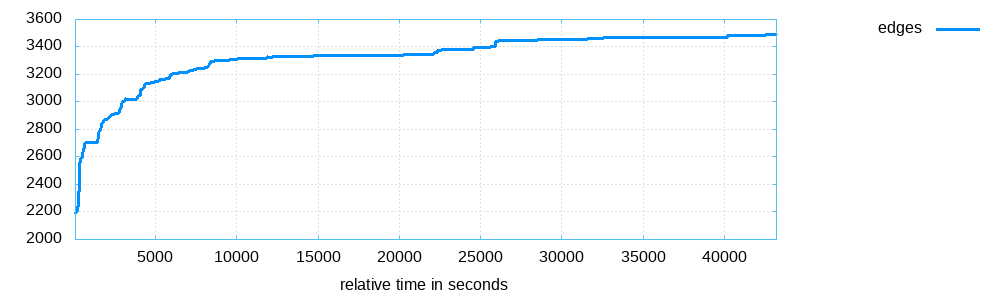
\includegraphics[width=\linewidth]{模糊测试-libass-第一轮-1.png}\end{minipage}\hfill
  \begin{minipage}{0.48\linewidth}\centering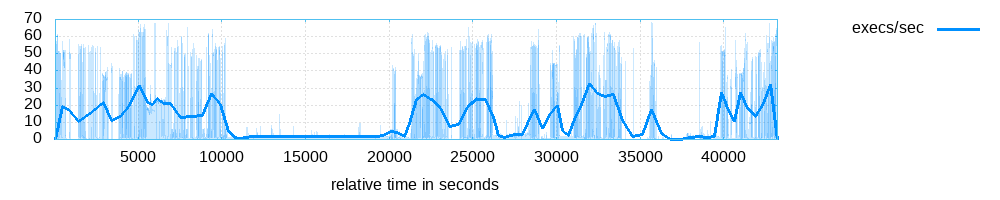
\includegraphics[width=\linewidth]{模糊测试-libass-第一轮-2.png}\end{minipage}

  \vspace{0.25em}
  \begin{minipage}{0.48\linewidth}\centering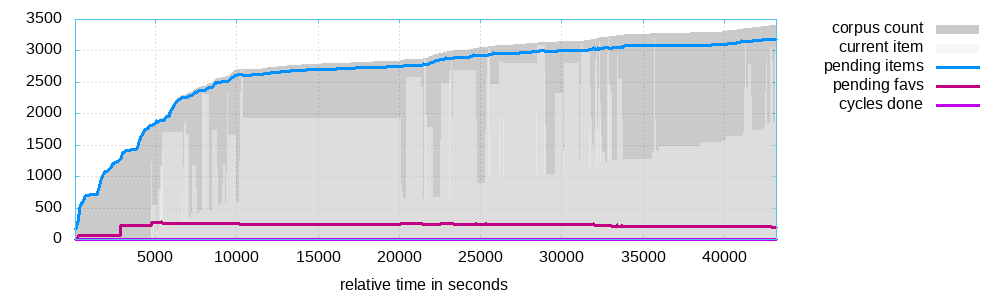
\includegraphics[width=\linewidth]{模糊测试-libass-第一轮-3.png}\end{minipage}\hfill
  \begin{minipage}{0.48\linewidth}\centering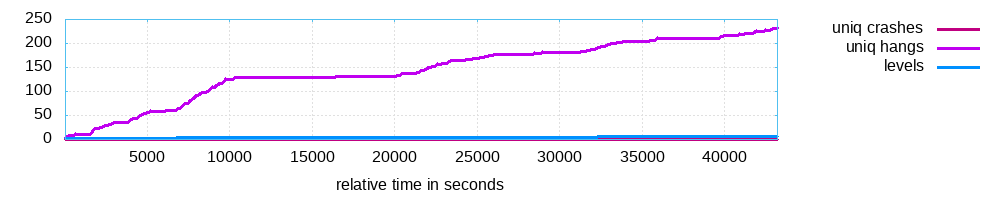
\includegraphics[width=\linewidth]{模糊测试-libass-第一轮-4.png}\end{minipage}
  \caption{libass 第一轮模糊测试截图（2×2 汇总）}
  \label{fig:libass-fuzz-round1}
\end{figure}

\begin{figure}[H]
  \centering
  \begin{minipage}{0.48\linewidth}\centering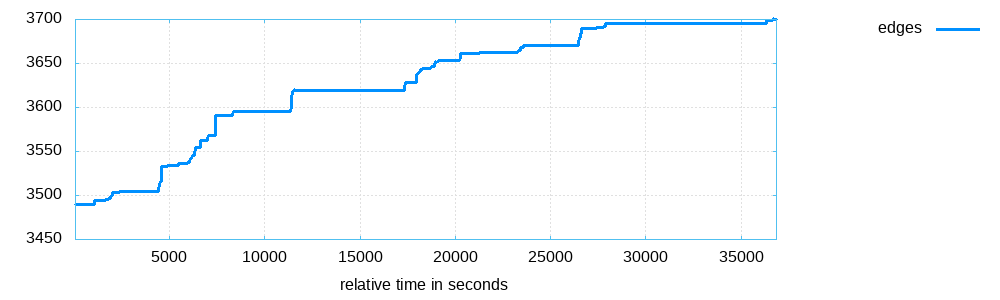
\includegraphics[width=\linewidth]{模糊测试-libass-第二轮-1.png}\end{minipage}\hfill
  \begin{minipage}{0.48\linewidth}\centering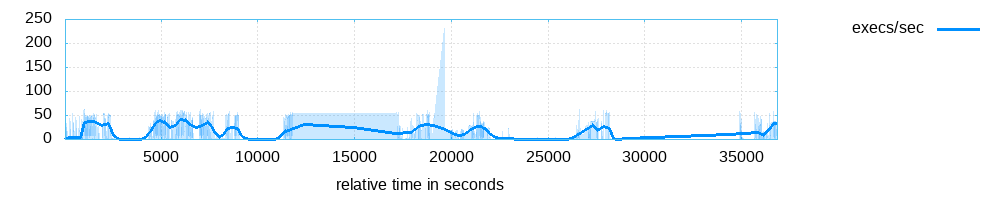
\includegraphics[width=\linewidth]{模糊测试-libass-第二轮-2.png}\end{minipage}

  \vspace{0.25em}
  \begin{minipage}{0.48\linewidth}\centering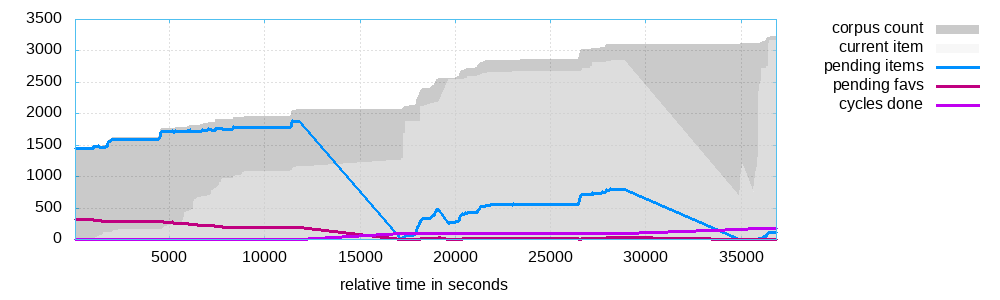
\includegraphics[width=\linewidth]{模糊测试-libass-第二轮-3.png}\end{minipage}\hfill
  \begin{minipage}{0.48\linewidth}\centering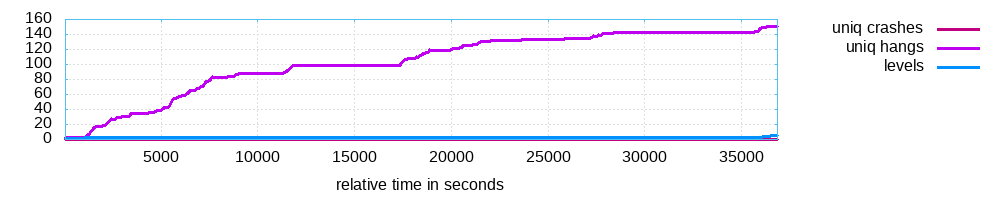
\includegraphics[width=\linewidth]{模糊测试-libass-第二轮-4.png}\end{minipage}
  \caption{libass 第二轮模糊测试截图（2×2 汇总）}
  \label{fig:libass-fuzz-round2}
\end{figure}

\begin{figure}[H]
  \centering
  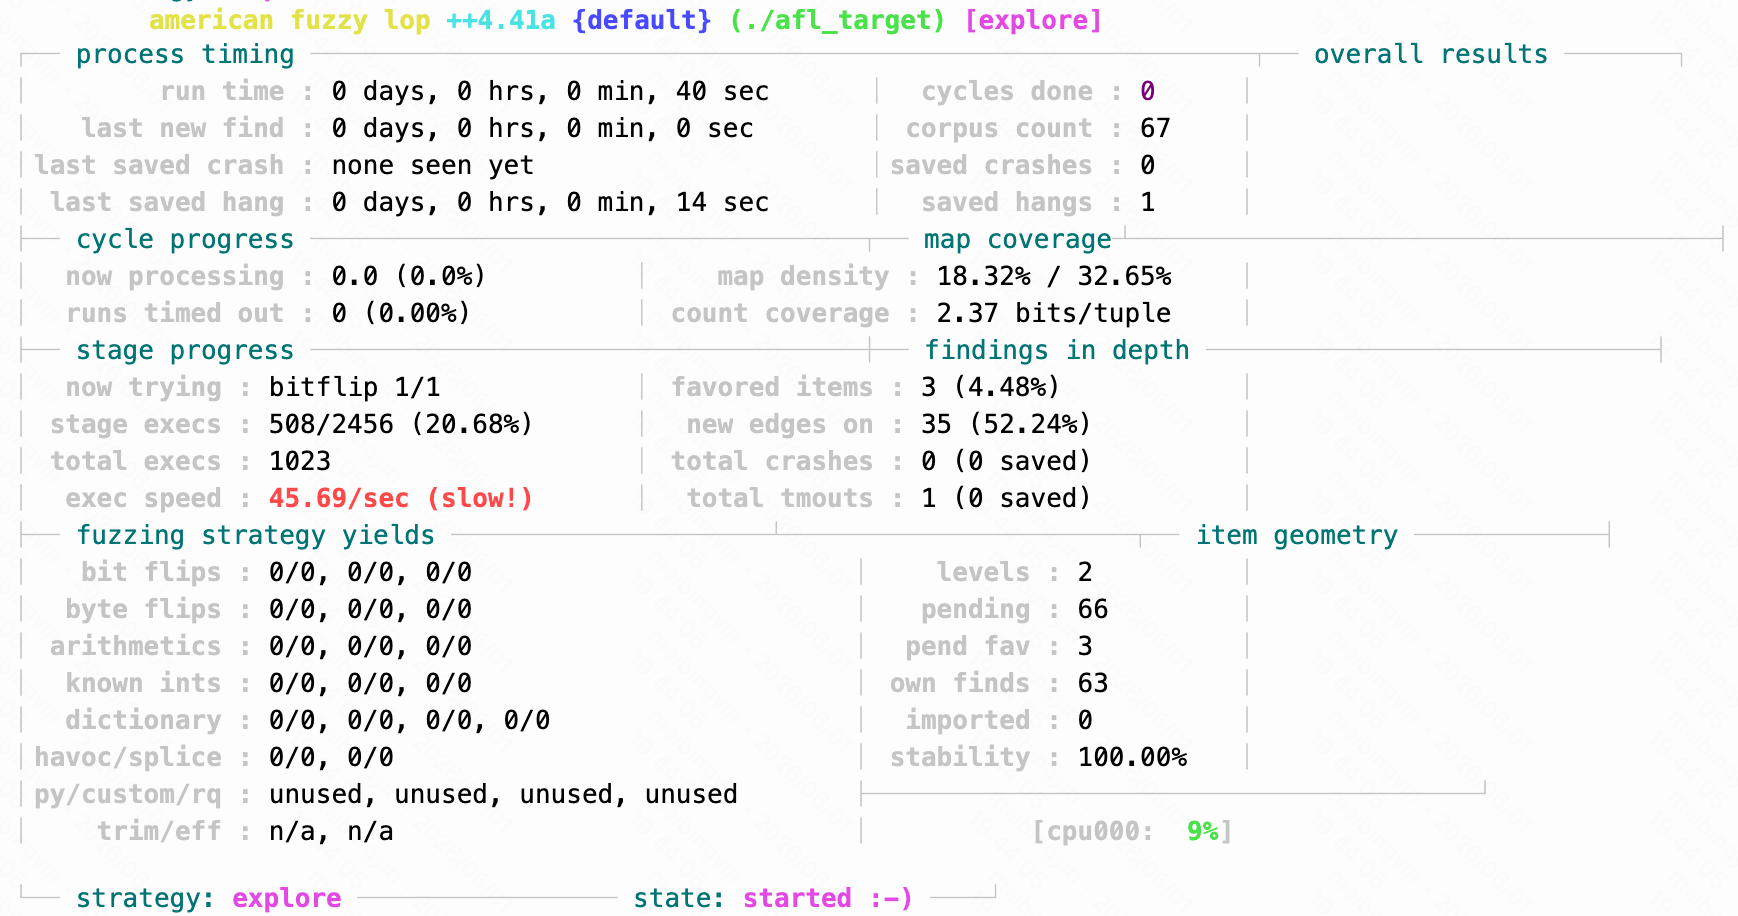
\includegraphics[width=0.9\linewidth]{模糊测试-libass-界面.png}
  \caption{libass 的 libFuzzer 与 AFL/AFL++ 动态测试界面}
  \label{fig:libass-fuzz-tools}
\end{figure}

\subsection{结果分析}
结合上述动态测试截图与运行日志，libass 方面的主要发现可按阶段归纳如下：
\begin{itemize}[leftmargin=2em]
  \item \textbf{第一轮：}单实例 + ASan 的 baseline 先跑通了基础渲染路径，覆盖率逐步提升至 53.59\%，共记录 233 个 hang；这些 hang 均与 \texttt{\textbackslash t()} 动画标签相关，证明 DoS 慢路径可独立复现。
  \item \textbf{第二轮：}为了突破第一轮只能到达浅层路径的瓶颈，我们引入结构感知 mutator 与 UBSan，对 \texttt{.ass} 语义字段做更细粒度变异，覆盖率继续提升，并发现 CWE-401、CWE-190、CWE-681 等问题，说明语义级变异对强格式输入尤为关键。
  \item \textbf{第三轮：}在第二轮已定位到矢量绘图边界点的基础上，针对 \texttt{\textbackslash p} 路径继续做专项强化，放大极端坐标与控制点输入，稳定复现整数溢出，但尚未将其推进为更深层的内存破坏。
  \item \textbf{第四轮：}为了独立验证 libFuzzer 发现的 DoS 慢路径，我们切换到 AFL++ 单实例 + ASan + 字典方案，用字典辅助变异并观察长时间运行下的表现，结果再次确认 hang 的主要来源就是 \texttt{\textbackslash t()} 路径。
  \item \textbf{第五轮：}针对第四轮字符串比较效率低、执行量不足的问题，我们引入 CMPLOG 与 4 核并行，让变异器能更好地学习关键字并共享语料，覆盖率提升到 56.82\%，总执行量达到 12,901,080 次，hang 数量进一步累积到 541，完成对 DoS 风险的二次确认。
\end{itemize}

表\ref{tab:libass-afl-summary}汇总了 AFL++ 分支两轮测试的整体结果，其中第二轮在执行次数和 hang 数量上均明显增加。

\begin{table}[H]
\centering
\caption{libass AFL 两轮测试结果汇总}
\label{tab:libass-afl-summary}
\begin{tabular}{lccccc}
\toprule
轮次 & edge 覆盖率 & 执行次数 & 语料库 & Crashes & Hangs \\
\midrule
第一轮：单实例 + ASan + 字典 & 53.59\% & 424,407 & 3,405 & 0 & 233 \\
第二轮：CMPLOG + 4 核并行 & 56.82\% & 12,901,080 & 3,227 & 0 & 541 \\
\bottomrule
\end{tabular}
\end{table}

表\ref{tab:libass-afl-parallel}进一步列出了 AFL++ 第二轮四个并行实例的结果，用于说明 CMPLOG 主实例和不同变异策略副实例之间的覆盖率与执行量差异。

\begin{table}[H]
\centering
\caption{libass AFL 第二轮并行实例结果}
\label{tab:libass-afl-parallel}
\begin{tabular}{lccc}
\toprule
实例 & 策略 & edge 覆盖率 & 执行次数 / Hangs \\
\midrule
main & CMPLOG & 56.82\% & 3,190,163 / 150 \\
slave1 & explore & 56.22\% & 3,213,452 / 134 \\
slave2 & exploit & 56.79\% & 3,273,489 / 129 \\
slave3 & fast & 56.77\% & 3,224,976 / 128 \\
合计 & — & — & 12,901,080 / 541 \\
\bottomrule
\end{tabular}
\end{table}

图\ref{fig:libass-flow}给出了 libass 实验流程的完整整理图，用于概括从静态分析、两条动态分支、五轮测试到 artifacts 汇总之间的整体链路。

\flowbox

\section{curl 项目评测}
curl 是一个成熟的网络传输库。相较于 libass，curl 的测试重点从复杂文本协议解析转向 URL 状态机、配置解析与网络异常处理。由于其输入与连接过程强相关，动态测试时常会出现可解析但无法完成连接的输入，从而形成大量 hang 或 timeout。图\ref{fig:curl-interface}展示了 curl 模糊测试过程中的运行界面。

\begin{figure}[H]
  \centering
  \begin{minipage}{0.48\linewidth}
    \centering
    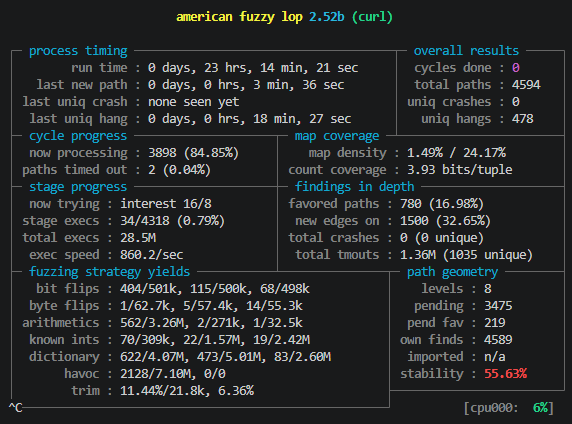
\includegraphics[width=\linewidth]{模糊测试-curl-界面.png}
    \caption{curl 模糊测试运行界面}
    \label{fig:curl-interface}
  \end{minipage}\hfill
  \begin{minipage}{0.48\linewidth}
    \centering
    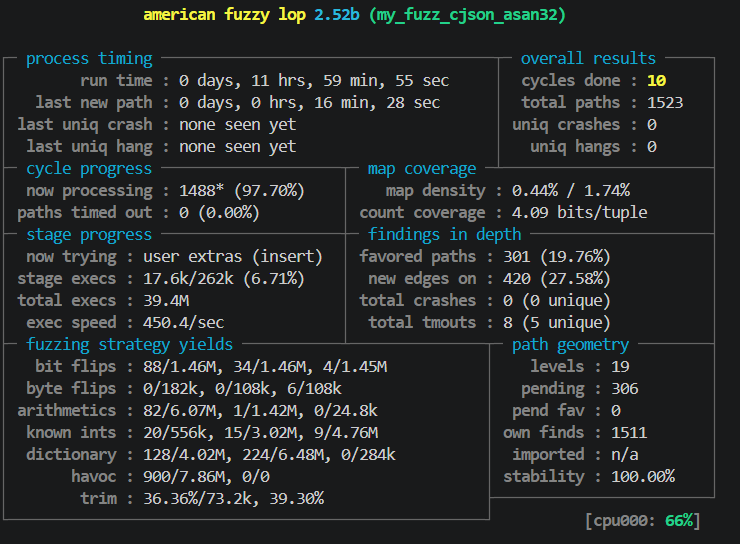
\includegraphics[width=\linewidth]{模糊测试-cjson-界面.png}
    \caption{cJSON 模糊测试运行界面}
    \label{fig:cjson-interface}
  \end{minipage}
\end{figure}

\subsection{静态分析结果}
curl 的静态分析主要采用 Clang Static Analyzer 的 scan-build。静态分析发现了一个较典型的资源释放问题：在配置文件解析路径中，非标准输入流在异常返回前未被正确关闭，存在潜在资源泄漏风险。这类问题在网络库与配置解析工具中较常见，尤其在处理批量异常输入时可能演化为文件描述符耗尽。图\ref{fig:curl-static}展示了 scan-build 对该问题的定位结果。

\begin{figure}[H]
  \centering
  \begin{minipage}{0.48\linewidth}\centering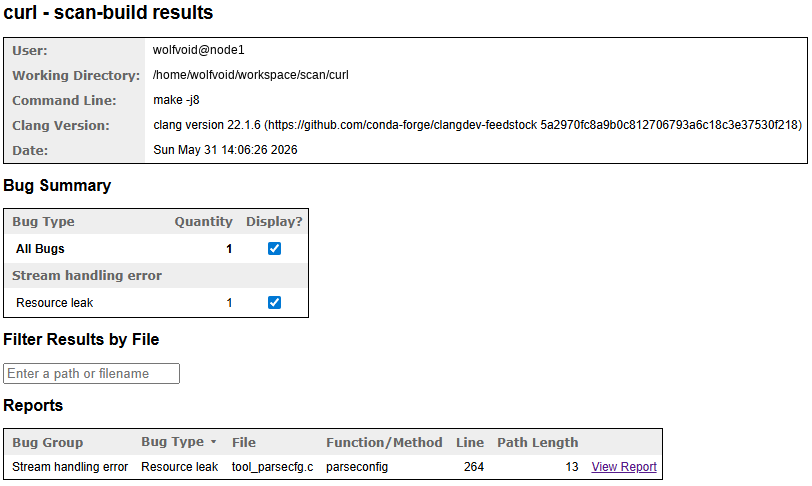
\includegraphics[width=\linewidth]{静态分析-curl-1.png}\end{minipage}\hfill
  \begin{minipage}{0.48\linewidth}\centering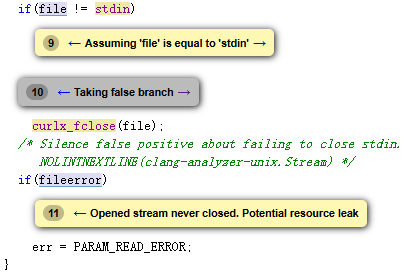
\includegraphics[width=\linewidth]{静态分析-curl-2.png}\end{minipage}
  \caption{curl 静态分析截图（双图并排）}
  \label{fig:curl-static}
\end{figure}

\subsection{动态测试方法}
我们使用 AFL++ 对 curl 进行动态测试，围绕 \texttt{parseconfig} 和 URL 状态机编写 harness，并引入 HTTP/SOCKS5 协议 token 字典，以提高对协议关键字、URL 组件和配置项分支的命中率。针对底层字符串比较较多的问题，我们启用 AFL++ 的 CMPLOG 机制，使变异器能够利用比较反馈突破字符串匹配瓶颈。整体测试累计超过 23 小时，执行次数约 28.5M 次。图\ref{fig:curl-dynamic}展示了 curl 动态模糊测试过程中的典型界面。

\begin{figure}[H]
  \centering
  \begin{minipage}{0.48\linewidth}\centering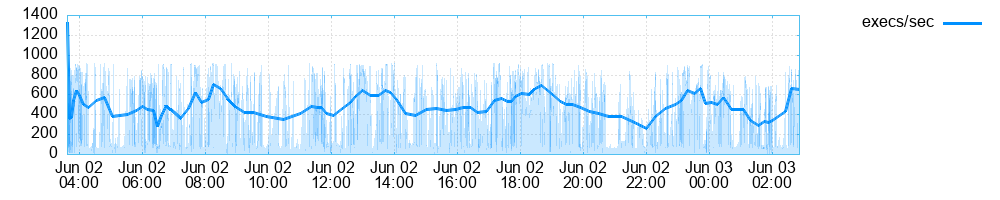
\includegraphics[width=\linewidth]{模糊测试-curl-1.png}\end{minipage}\hfill
  \begin{minipage}{0.48\linewidth}\centering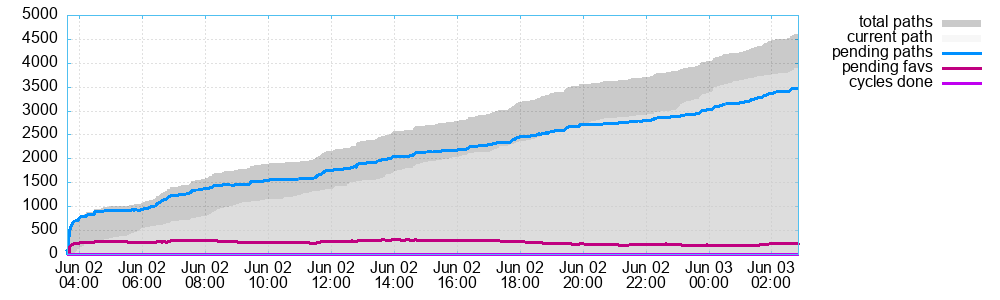
\includegraphics[width=\linewidth]{模糊测试-curl-2.png}\end{minipage}

  \vspace{0.25em}
  \begin{minipage}{0.48\linewidth}\centering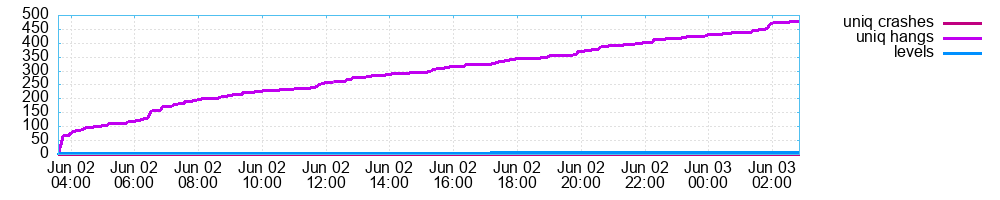
\includegraphics[width=\linewidth]{模糊测试-curl-3.png}\end{minipage}\hfill
  \begin{minipage}{0.48\linewidth}\centering\phantom{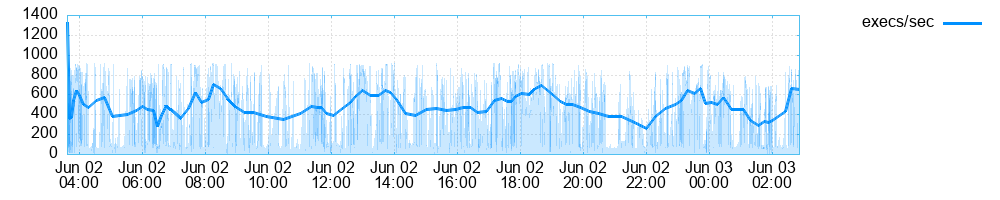
\includegraphics[width=\linewidth]{模糊测试-curl-1.png}}\end{minipage}
  \caption{curl 动态测试截图}
  \label{fig:curl-dynamic}
\end{figure}

\subsection{结果分析}
综合静态分析与动态测试结果，curl 这一部分的主要结论如下：
\begin{itemize}[leftmargin=2em]
  \item \textbf{CWE-404 资源泄漏：}问题位于 \texttt{tool\_parsecfg.c} 第 264 行。在打开非标准输入流（\texttt{file != stdin}）后，如果 \texttt{fileerror} 检测为真，程序会进入错误处理分支并直接返回 \texttt{PARAM\_READ\_ERROR}，从而错过函数末尾的 \texttt{fclose(file)} 操作。
  \item \textbf{影响分析：}在处理海量畸形配置文件时，上述路径可能导致文件描述符持续泄漏，最终触发 FD 耗尽，造成程序异常退出或拒绝服务。
  \item \textbf{动态测试现象：}AFL++ 测试中主要观察到 hang 或 timeout，而非稳定 crash。这与网络类库的工程特征一致：输入可能已经通过解析层，但在真实连接、重试或等待阶段被阻塞。
  \item \textbf{总体判断：}curl 作为成熟网络库，核心路径稳定性较好；本次实验中更值得关注的是异常配置解析路径上的资源管理问题，而不是传统内存破坏型崩溃。
\end{itemize}

\section{cJSON 项目评测}
cJSON 是一个轻量级 JSON 解析库。与 libass 相比，cJSON 的输入结构更清晰、协议更简单，因此更适合通过逐轮扩展 harness 的方式提高覆盖率。图\ref{fig:cjson-interface}展示了 cJSON 模糊测试过程中的运行界面。

\subsection{静态检查结果}
cJSON 采用 cppcheck 进行静态检查，共获得 121 条诊断信息。经排查，这些告警主要来自跨平台宏定义和编译环境差异，例如 \texttt{NAN} 重定义等情况，未形成可确认的实际漏洞。

\subsection{动态测试过程}
我们对 cJSON 采用三轮递进式动态评测方法。第一轮使用 cJSON 官方 AFL harness 和基础 JSON 种子，以 \texttt{./fuzz\_cjson @@} 运行 baseline 测试，主要覆盖 JSON 解析路径，最终 \texttt{cJSON.c} 行覆盖率为 24.93\%。

第二轮在 AFL 2.52b 中加入 ASAN，并编写自定义 driver，通过输入前 4 字节控制测试模式，覆盖 \texttt{cJSON\_Parse}、\texttt{cJSON\_ParseWithOpts}、格式化/非格式化打印、buffered print、minify 和释放逻辑。同时，我们加入合法 JSON、非法 JSON、边界数字、转义字符串等种子，使 \texttt{cJSON.c} 行覆盖率提升至 47.01\%。

第三轮使用 AFL++ 4.33c、ASAN、CMPLOG 和 4 实例并行 fuzz，进一步扩展 driver，覆盖对象/数组增删改、类型判断、duplicate/compare、preallocated print，以及 \texttt{cJSON\_Utils} 中的 pointer、patch、merge、sort 等 API。测试结束后，我们进行语料精简和 gcov 回放，最终 \texttt{cJSON.c} 行覆盖率提升至 86.97\%，\texttt{cJSON\_Utils.c} 行覆盖率达到 76.96\%，总体行覆盖率达到 85.18\%。图\ref{fig:cjson-rounds}展示了第二轮测试过程中的典型截图，图\ref{fig:cjson-round3}展示了第三轮并行 fuzz 与覆盖率回放阶段的截图，图\ref{fig:cjson-afl-code}进一步展示了动态测试界面与相关代码情况。

\begin{figure}[H]
  \centering
  \begin{minipage}{0.48\linewidth}\centering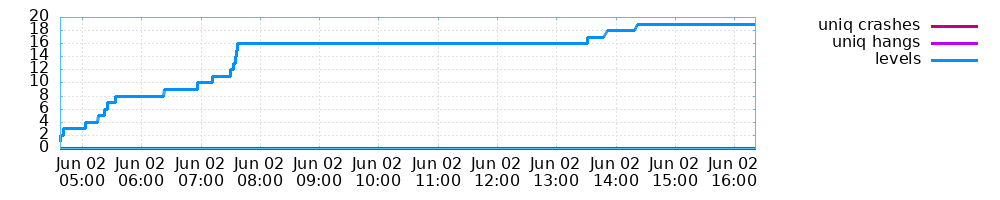
\includegraphics[width=\linewidth]{模糊测试-cjson-第二轮-1.png}\end{minipage}\hfill
  \begin{minipage}{0.48\linewidth}\centering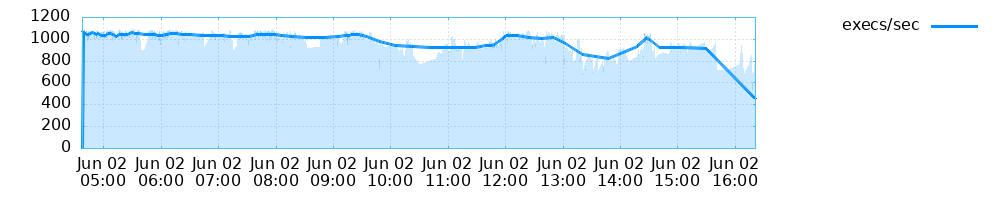
\includegraphics[width=\linewidth]{模糊测试-cjson-第二轮-2.png}\end{minipage}

  \vspace{0.25em}
  \begin{minipage}{0.48\linewidth}\centering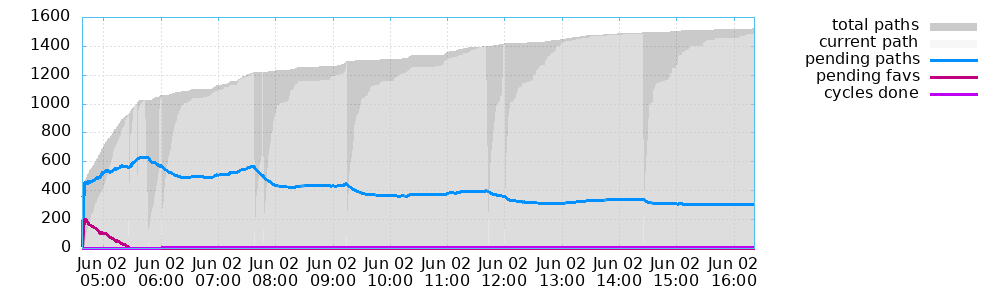
\includegraphics[width=\linewidth]{模糊测试-cjson-第二轮-3.png}\end{minipage}\hfill
  \begin{minipage}{0.48\linewidth}\centering\phantom{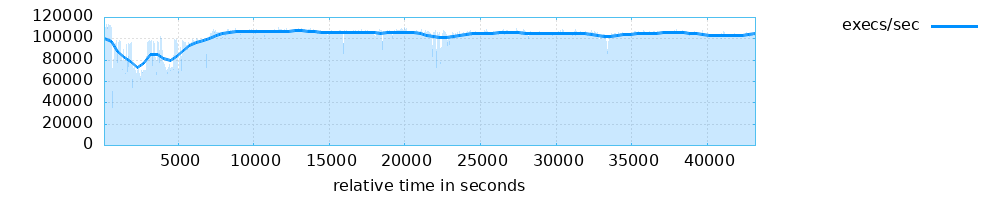
\includegraphics[width=\linewidth]{模糊测试-cjson-第三轮-3.png}}\end{minipage}
  \caption{cJSON 第二轮模糊测试截图（2×2 汇总）}
  \label{fig:cjson-rounds}
\end{figure}

\begin{figure}[H]
  \centering
  \begin{minipage}{0.48\linewidth}\centering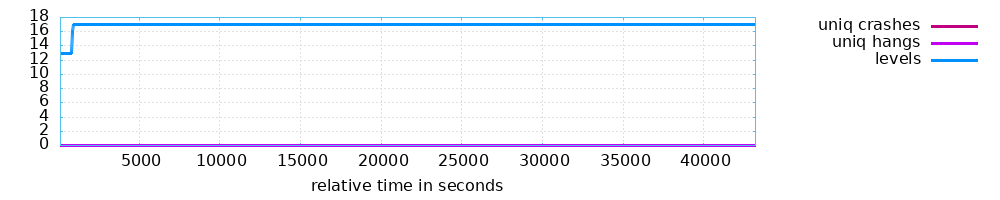
\includegraphics[width=\linewidth]{模糊测试-cjson-第三轮-1.png}\end{minipage}\hfill
  \begin{minipage}{0.48\linewidth}\centering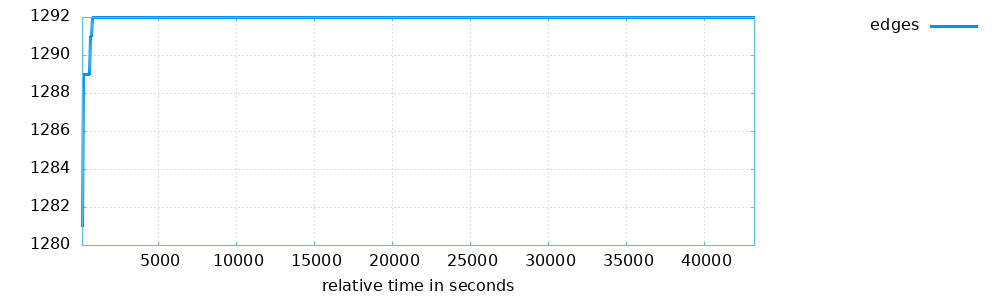
\includegraphics[width=\linewidth]{模糊测试-cjson-第三轮-2.png}\end{minipage}

  \vspace{0.25em}
  \begin{minipage}{0.48\linewidth}\centering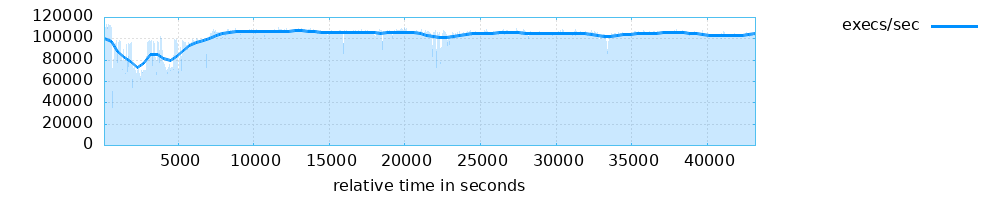
\includegraphics[width=\linewidth]{模糊测试-cjson-第三轮-3.png}\end{minipage}\hfill
  \begin{minipage}{0.48\linewidth}\centering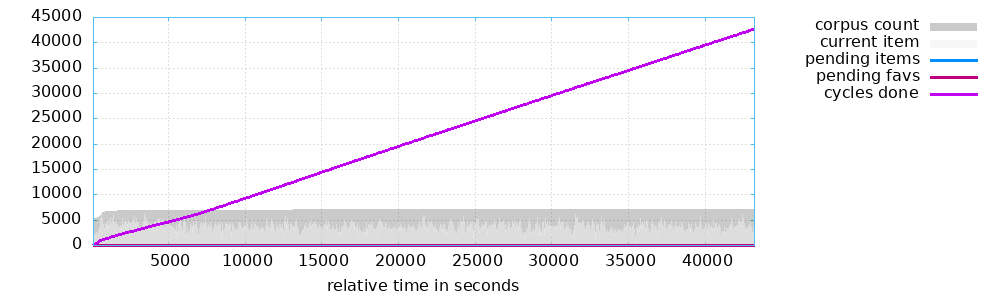
\includegraphics[width=\linewidth]{模糊测试-cjson-第三轮-4.png}\end{minipage}
  \caption{cJSON 第三轮模糊测试截图（2×2 汇总）}
  \label{fig:cjson-round3}
\end{figure}

\begin{figure}[H]
  \centering
  \begin{minipage}[t]{0.30\linewidth}\vspace{0pt}\centering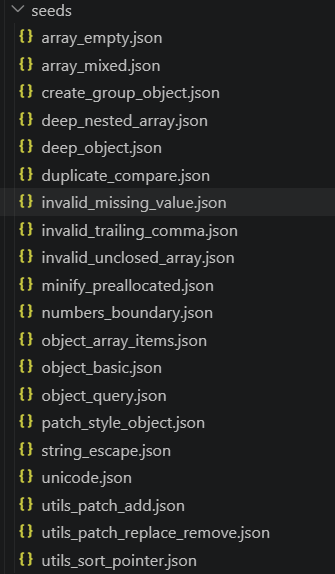
\includegraphics[width=\linewidth]{动态分析-cjson-afl-1.png}\end{minipage}\hfill
  \begin{minipage}[t]{0.64\linewidth}\vspace{0pt}\centering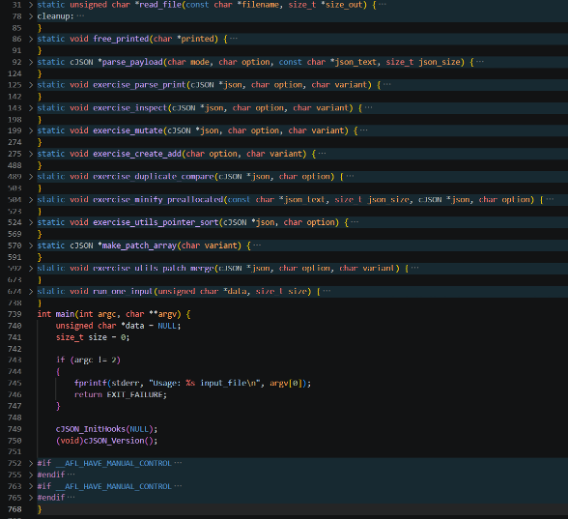
\includegraphics[width=\linewidth]{cjson-code.png}\end{minipage}
  \caption{cJSON 动态测试界面与代码截图}
  \label{fig:cjson-afl-code}
\end{figure}


\subsection{结果分析}
经 12 小时高强度并发测试，cJSON 动态测试结果为 0 Crashes、0 Hangs。结合静态检查结果可以看出，虽然 cppcheck 产生了 121 条告警，但经排查均为跨平台宏定义或工具环境差异带来的误报，未发现可稳定复现的安全问题。

未发现问题的主要原因在于，cJSON 作为成熟的底层解析库，代码规模较小、维护时间较长，核心状态机对指针越界和 Null 引用具有较严格的防御。与此同时，传统“盲变异”难以有效破坏 JSON 的严格层级结构，容易在语法层面被快速拒绝。后续若继续提高评测深度，建议引入 Structure-Aware Fuzzing（结构感知变异），例如利用 libprotobuf-mutator 约束 Fuzzer 生成语法正确的 JSON 树，从而探索更深层的逻辑分支。

\section{Agent 辅助工作设计与实现}
针对传统漏洞挖掘中“测试桩编写成本高”、“日志清洗与误报率高”的痛点，我们设计并实现了一个基于 LLM 的漏洞挖掘 Agent 辅助与编排工作站。采用动静结合协同模式：Agent 不替代 Fuzzer 执行代码，而是作为工程师的分析助手，辅助完成测试桩生成、静态报告降噪和动态日志分诊等高重复度工作。

在工具与模型选型上，工作站底座接入 SiliconFlow 平台，并采用 DeepSeek-V3 大语言模型 API 进行核心逻辑推理；前端使用 HTML5 与 Fetch 构建 Agent 控制台界面，使其能够接收源码切片、静态分析日志和动态测试堆栈，并将传递到后续流程中。

本工作站分为以下三部分，实现 AI 与静态分析、动态测试工具的结合：
\begin{itemize}[leftmargin=2em]
  \item \textbf{前置辅助：靶点与字典生成。}在本地离线测试开始前，我们将项目真实 C 源码的抽象语法树（AST）切片输入 Agent。模型通过阅读源码，自动输出对应的 \texttt{LLVMFuzzer TestOneInput} 初始化代码结构，并提取代码中的常量字符串，生成面向目标项目的专属变异字典。图\ref{fig:agent-libass-harness}展示了 Agent 辅助构建 libass 初始化测试桩的结果。
  \item \textbf{后期清洗：静态报告降噪。}对于 scan-build 和 cppcheck 产生的大量冗杂日志，Agent 利用大模型的语义理解能力过滤跨平台兼容性、宏定义差异等误报（False Positives），并提炼更值得人工确认的问题。例如在 curl 评测中，Agent 辅助定位并输出了与 \texttt{tool\_parsecfg.c} 相关的 CWE-404 资源泄漏风险，如图\ref{fig:agent-curl-cwe404}所示。
  \item \textbf{后期清洗：动态日志分诊与 RCA。}AFL++ 会产出大量 crash/hang 日志，ASan/UBSan 也会生成较长的原始堆栈（Raw Stack Trace）。我们将这些堆栈和运行摘要挂载给 Agent，由其自动执行崩溃去重和根因分析（Root Cause Analysis）。例如在 libass 测试中，Agent 能够将大量 hang 归因到特定标签触发的算法复杂度缺陷，从而减少人工溯源时间。
\end{itemize}

\begin{figure}[H]
  \centering
  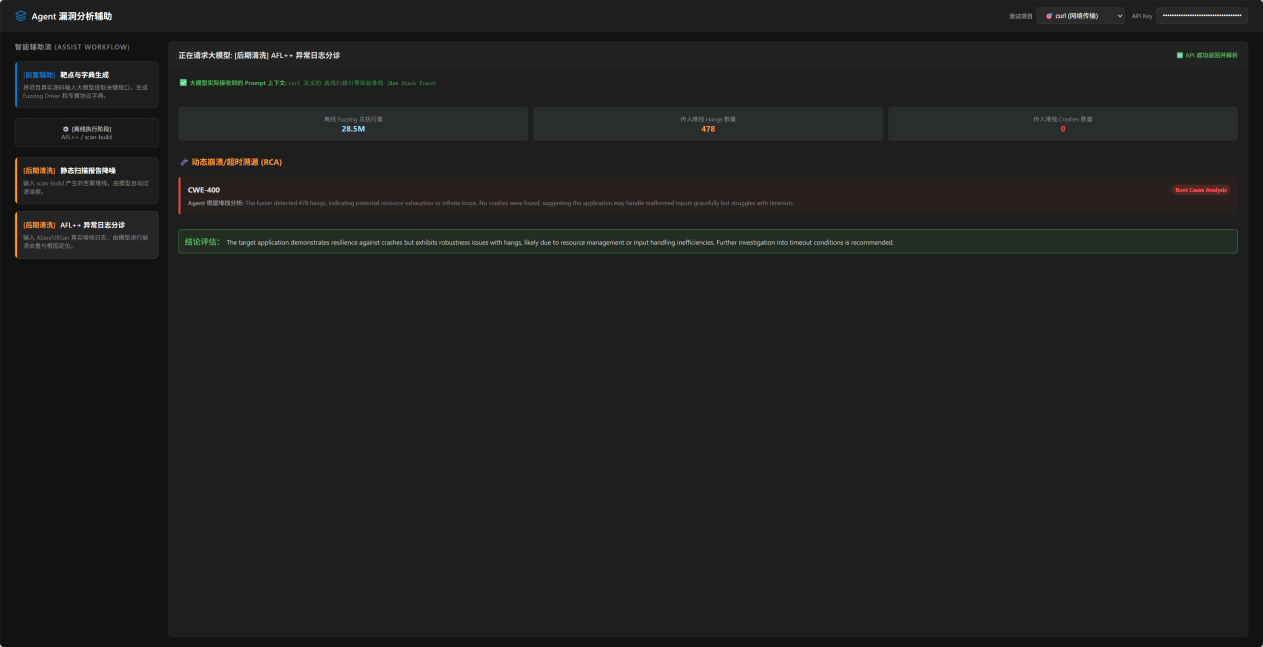
\includegraphics[width=0.93\linewidth]{agent-curl-cwe404.png}
  \caption{输出 curl 的 CWE-404}
  \label{fig:agent-curl-cwe404}
\end{figure}

\begin{figure}[H]
  \centering
  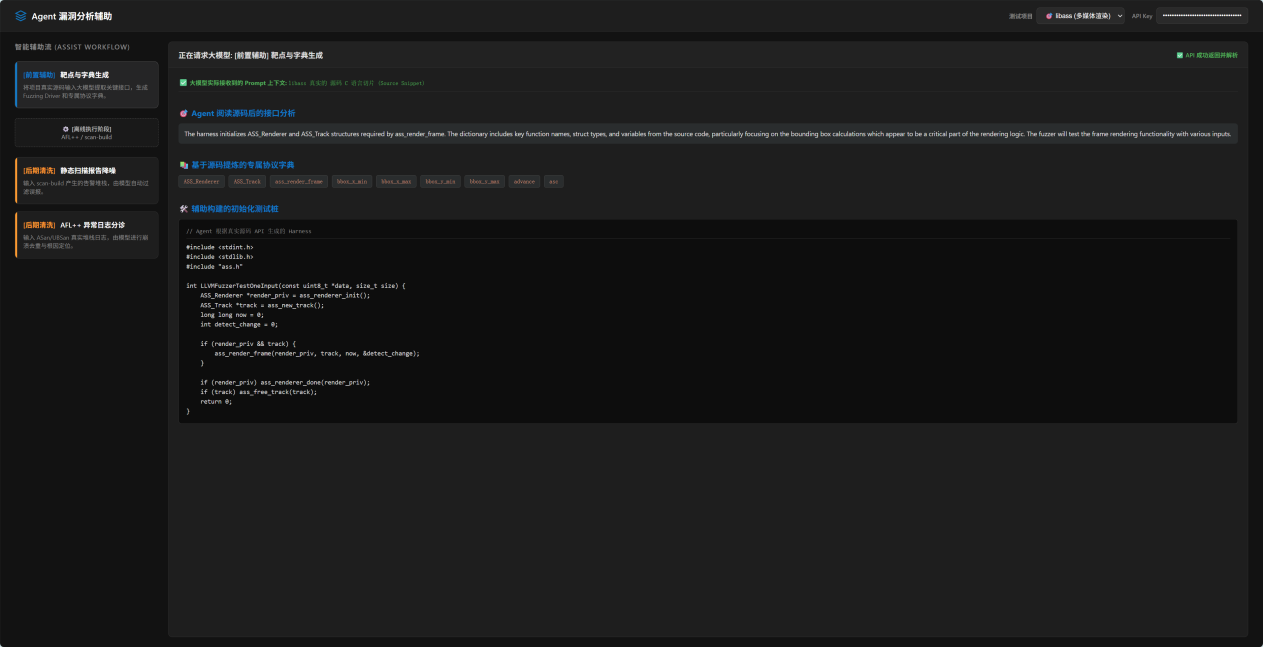
\includegraphics[width=0.93\linewidth]{agent-libass-harness.png}
  \caption{辅助构建 libass 的初始化测试桩}
  \label{fig:agent-libass-harness}
\end{figure}
\section{实验总结}
通过本次实验，我们对三个不同类型的开源项目进行了静态分析与动态模糊测试的联合评测，获得了较有代表性的结论。libass 更适合通过结构感知 fuzzing 挖掘复杂渲染路径中的边界问题；curl 更能体现网络库在异常状态和资源管理方面的风险；cJSON 则说明了 driver 设计和语料质量对覆盖率的决定性影响。

总体而言，本次实验让我们更直观地体会到，漏洞挖掘并不是单纯依赖工具长时间运行即可完成的任务，而是需要将测试桩设计、语料构造、覆盖率反馈、日志分析和人工判断结合起来。不同项目的输入结构和工程特征差异很大，适用的 fuzzing 策略也不同；只有理解目标程序的解析逻辑和关键路径，才能更有效地提升测试深度。同时，Agent 辅助分析也让我们认识到，自动化工具在降噪、归纳和溯源方面能够显著提高实验效率，但最终结论仍需要结合源码和运行结果进行人工确认。

\begin{thebibliography}{9}
\bibitem{libass} libass 项目主页：\url{https://github.com/libass/libass}
\bibitem{curl} curl 项目主页：\url{https://github.com/curl/curl}
\bibitem{cjson} cJSON 项目主页：\url{https://github.com/DaveGamble/cJSON}
\bibitem{aflpp} AFL++ 官方文档：\url{https://github.com/AFLplusplus/AFLplusplus}
\bibitem{cppcheck} cppcheck 官方文档：\url{https://cppcheck.sourceforge.io/}
\end{thebibliography}

\end{document}
